\chapter{Extensions of the HH4b Search}
\label{chap:eight}



\section{VBF Production of HH in the 4b Final State \label{s:vbf}}

\begin{figure} %  figure placement: here, top, bottom, or page
    \centering
 %   
\includegraphics[width=\textwidth,height=\textheight,keepaspectratio]{fig_2-1}
    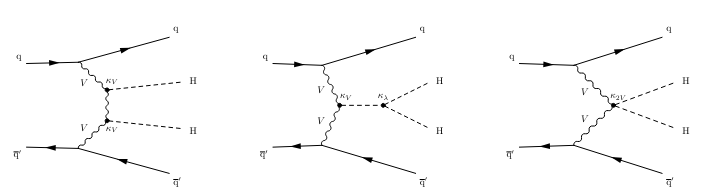
\includegraphics[scale=0.6]{vbffyenman.png}
    \caption{Feynman diagrams for Vector Boson Fusion production of HH in the 4b Final State.}
    \label{fig:vbffeynman}
 \end{figure}


The previously described analysis of boosted HH in the 4b final state focuses on the dominant HH production mode, gluon-gluon fusion (ggF).
This is not the only production mode that can be studied. The next most common production mode is through vector boson fusion (VBF).
The importance of this production mode is that the leading order diagrams provide a way to measure the Higgs self-coupling (HHH), the vector boson coupling (VVH), and the quartic HHVV coupling.
These are called, $\kappa_{\lambda}$, $\kappa_V$, and $\kappa_{2V}$ respectively.
While the other two couplings, $\kappa_{\lambda}$ and $\kappa_V$, are able to be probed by other methods, the quartic coupling, $\kappa_{2V}$ is uniquely probed by the VBF production mode.
According to the SM, all of these coupling should all be equal to 1.

At energy scales available at the LHC, the leading contribution for longitudinal scattering amplitude of the VBF production is found to be proportional to $m_{HH}$ times $\kappa_{2V} - \kappa_V^2$, where $m_{HH}$ is the invariant mass of the di-Higgs system. 
This means that in the SM, the two leftmost diagrams of Figure \ref{fig:vbffeynman} cancel each other almost completely (since $\kappa_{2V} = \kappa_V = 1$), yielding a small production cross section. 
However, in more generic models where $\kappa_{2V} \neq 1$ and/or $\kappa_V \neq 1$, this is not the case and the VBF cross section is dramatically increased, especially in phase space region characterized by large di-Higgs invariant mass. 

This analysis then attempts to set stricter limits on $\kappa_{2V}$ by using a novel, powerful multivariate classifier based on graph neural networks, the \textit{ParticleNet} jet tagger.
In addition to flavor tagging, the ParticleNet DNN architecture is also applied to train a jet mass regression algorithm, allowing efficient background suppression based on the regressed mass of the $H \rightarrow bb$ candidate jets.
The statistical tests and systematic uncertainties used in this analysis are adapted in part or whole from the HH to 4b search.

Here we show the limits placed on $\kappa_{2V}$.
\begin{figure} %  figure placement: here, top, bottom, or page
    \centering
 %   
\includegraphics[width=\textwidth,height=\textheight,keepaspectratio]{fig_2-1}
    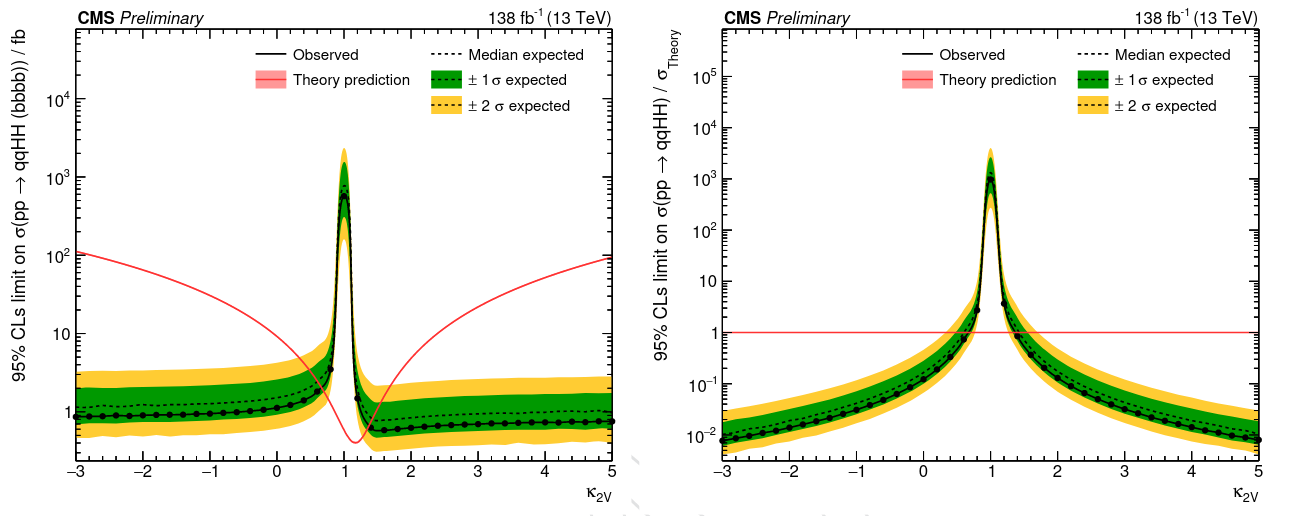
\includegraphics[scale=0.35]{kappa2vlimit.png}
    \caption{Expected and observed 95\% CL exclusion limit on the product of the HH production cross section and the branching fraction into the 4b final state, as a function of the κ2V
    coupling, obtained using the Asimov dataset. The crossings of expected median (dashed black
    line) and the theoretical cross section (red line) indicate the expected range of the $\kappa_{2V}$ values to
    be excluded at 95\% CL}
    \label{fig:kappa2Vlimit}
 \end{figure}

 \begin{figure} %  figure placement: here, top, bottom, or page
    \centering
 %   
\includegraphics[width=\textwidth,height=\textheight,keepaspectratio]{fig_2-1}
    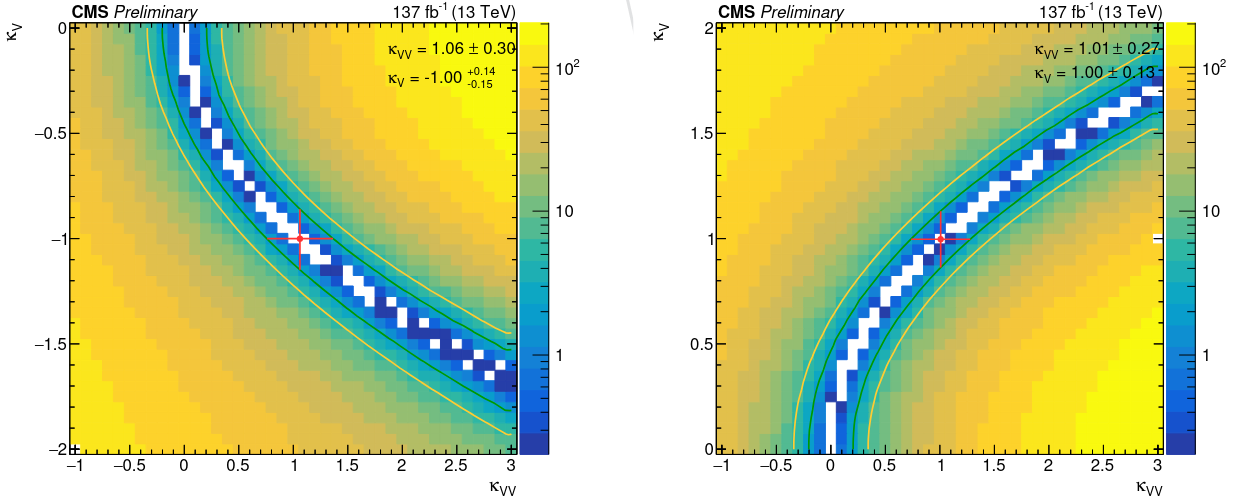
\includegraphics[scale=0.35]{kappa2vscan.png}
    \caption{Two-dimensional likelihood scan where both $\kappa_{2V}$and $\kappa_{V}$ couplings are varied simultaneously, for $\kappa_{V} < 0$ (left) and $\kappa_{V} > 0$ (right)}
    \label{fig:kappa2Vscan}
 \end{figure}

\section{A Massive Resonance decaying to a light scalar and a Higgs Boson in the 4b Final State}

\begin{figure} %  figure placement: here, top, bottom, or page
    \centering
 %   
\includegraphics[width=\textwidth,height=\textheight,keepaspectratio]{fig_2-1}
    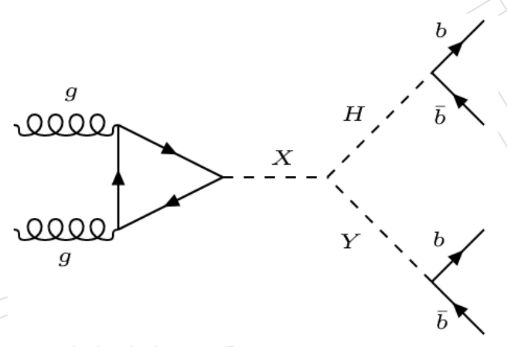
\includegraphics[scale=0.5]{ggfHY.png}
    \caption{Feynman diagram for gluon gluon fusion production of HY in the 4b Final State.}
    \label{fig:hy4bfeynman}
 \end{figure}


One class of searches is the search for additional spin-0 (scalar) particles. These are motivated in the two-Higgs doublet models which extend the SM scalar sector by one additional scalar doublet. 
In particular, the type II two-Higgs doublet model such as the Minimal Supersymmetric extension of the standard model (MSSM) postulates the existence of extra CP even scalars (H and h) and CP-odd pseudo-scalars (A) with sizable production cross sections. 
One of these could be the discovered Higgs boson $H_{125}$. The next-to-Minimal Supersymmetric extension of the standard model (NMSSM) contains an additional scalar complex singlet which mixes with the existing scalar doublets to give rise to extra CP-even and CP-odd states with masses below the scale of the heavier scalars. 
Thus, in these models, cascade decays such as $H \rightarrow H_{125}H_{125}$ or $H \rightarrow hH_{125}$ are possible, if kinematically favorable.

As the $H \rightarrow H_{125}H_{125}$ is the main search of this thesis, one can then probe the $H \rightarrow hH_{125}$ decay.
The cascade production and decay processes involving two new scalars of unequal masses $pp \rightarrow X \rightarrow HY$, X being the heavier and Y being the lighter scalars, are yet to be explored at the LHC, though several searches are ongoing or planned. 
One of the main difficulties of such a search, compared with final states having two particles of equal masses, is the reconstruction of the two different mass particles. 
Overall, the physics signature will have two unknown masses, that of the parent massive resonance X and that of the undiscovered scalar Y.
The H and Y candidates are selected by employing jet tagging techniques, including the previously mentioned ParticleNet, to identify jets consistent with the decay of a massive resonance into a pair of b quarks.
The background estimate method, statistical tests, and systematic uncertainties used in this analysis are adapted in part or whole from the HH to 4b search.

As of the writing of this thesis, the final results if this HY to 4b search have not been made public so here we show the expected limits on both $M_X$ and $M_Y$.

\begin{figure} %  figure placement: here, top, bottom, or page
    \centering
 %   
\includegraphics[width=\textwidth,height=\textheight,keepaspectratio]{fig_2-1}
    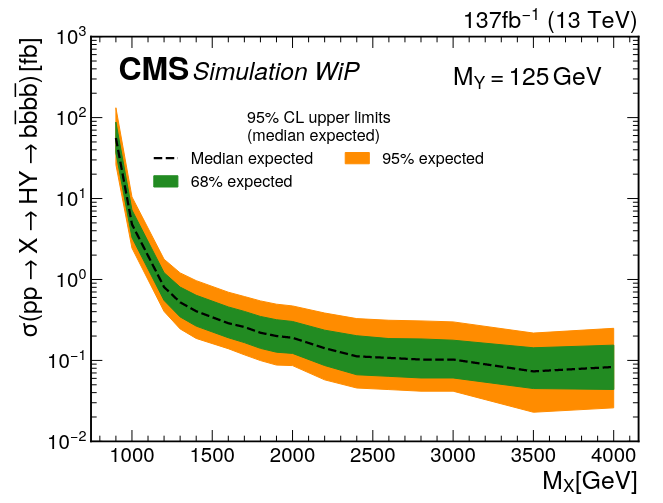
\includegraphics[scale=0.5]{hy4b125limit.png}
    \caption{The expected upper limit of $pp \rightarrow HY \rightarrow b\bar{b} b\bar{b}$ at 95\% confidence level for a fixed mass of Y, $M_Y = 125 GeV$. Calculated using toy data for full RunII.}
    \label{fig:hy4b125limit}
 \end{figure}

 \begin{figure} %  figure placement: here, top, bottom, or page
    \centering
 %   
\includegraphics[width=\textwidth,height=\textheight,keepaspectratio]{fig_2-1}
    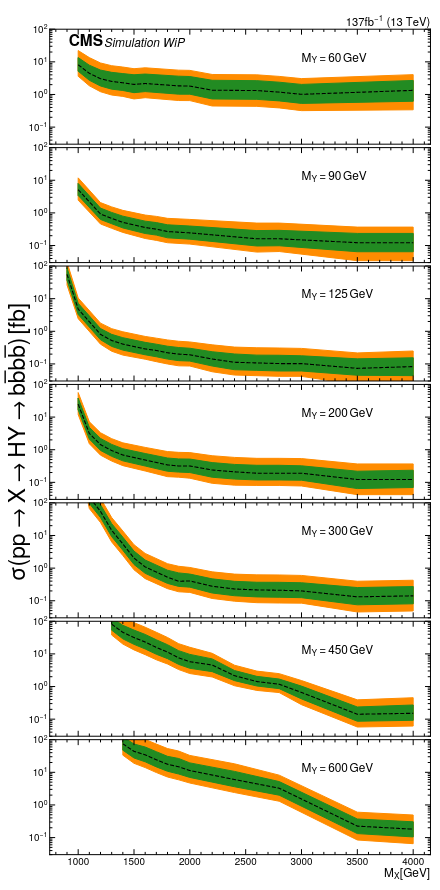
\includegraphics[scale=0.65]{hy4blimit.png}
    \caption{The expected upper limit of $pp \rightarrow HY \rightarrow b\bar{b} b\bar{b}$ at 95\% confidence level for seven different $M_Y$. Limits are calculated using toy data for full RunII}
    \label{fig:hy4blimit}
 \end{figure}

 \begin{figure} %  figure placement: here, top, bottom, or page
    \centering
 %   
\includegraphics[width=\textwidth,height=\textheight,keepaspectratio]{fig_2-1}
    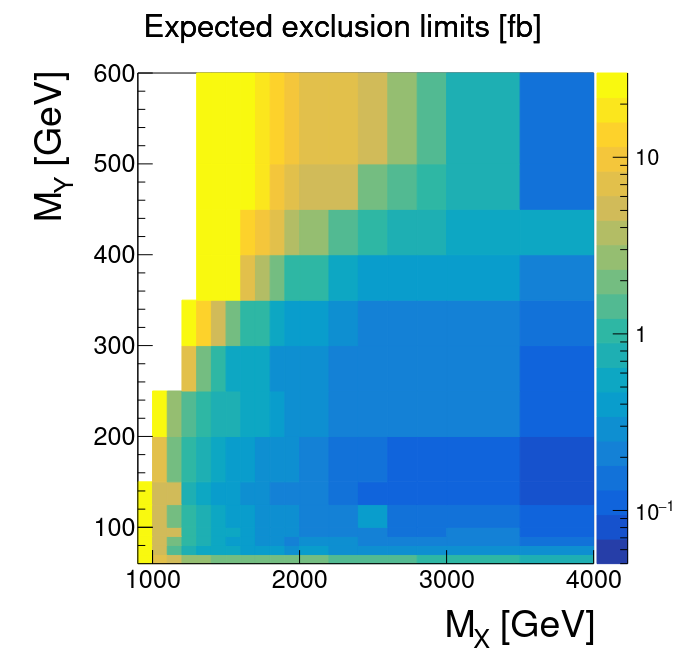
\includegraphics[scale=0.5]{hy4b2dlimit.png}
    \caption{The expected upper limit of $pp \rightarrow HY \rightarrow b\bar{b} b\bar{b}$ at 95\% confidence level in the $M_X, M_Y$ plane. Limits are calculated using toy data for full RunII.}
    \label{fig:hy4b2dlimit}
 \end{figure}